

Lai demonstrētu \Gls{snn} detektora praktisko piemērotību, impulsu konvolūcijas pamattīkls realizēts pārkonfigurējamajā \Gls{fpga} paātrinātājā, kas aprakstīts \ref{sec:fpga_impl}. apakšnodaļā. Aparatūras realizācijā izmantota tā pati tīkla topoloģija kā \textit{SpikingJelly} ietvarā izstrādātajam programmatūras modelim, lai saglabātu līdzvērtību starp programmatūras apmācību un aparatūras inferenci. Paātrinātājs atbalsta konvolūcijas slāņus ar līdz 256 ieejas un 512 izejas kanāliem, ļaujot realizēt dziļus tīklus praktiskiem lietojumiem.

Arhitektūra ir konfigurējama pazīmju kartēm līdz \(512 \times 512\) pikseļiem, kas atbilst vokseļu režģiem apkārtskata uztverei aptuveni \qty{50}{\metre} rādiusā ar horizontālo vokseļu izšķirtspēju līdz \qty{0.1}{\metre}. Tādējādi tā pati paātrinātāja arhitektūra bez aparatūras izmaiņām var izpildīt gan kompaktos novērtēšanas tīklus, gan lielākus 3D objektu detektēšanas modeļus.

\ref{fig:fpga_vs_jetson}. attēlā salīdzināts izmērītais \Gls{fpga} realizācijas inferences latentums ar ekvivalentu programmatūras realizāciju \textit{Jetson AGX Orin} GPU, kur \Gls{fpga} un \textit{Jetson} izpilda vienādu impulsu tīkla konfigurāciju ar vienādiem ieejas izmēriem un laika soļu skaitu. Norādītais \Gls{fpga} latentums aptver impulsu konvolūcijas pamattīkla izpildi un neietver ieejas vokselizāciju, \Gls{ssd} detektēšanas galvas apstrādi un ietverošo taisnstūru pēcapstrādi. Tā kā \Gls{fpga} apstrādā konvolūcijas slāņus kā konveijerizētu datu straumi, pievienojot tīklam papildu slāņus, latentums palielinās tikai nedaudz. Savukārt GPU izpildes laiks pieaug aptuveni proporcionāli tīkla dziļumam, jo katrs slānis tiek izpildīts kā atsevišķs kodols.

\begin{figure}[ht]
  \centering
  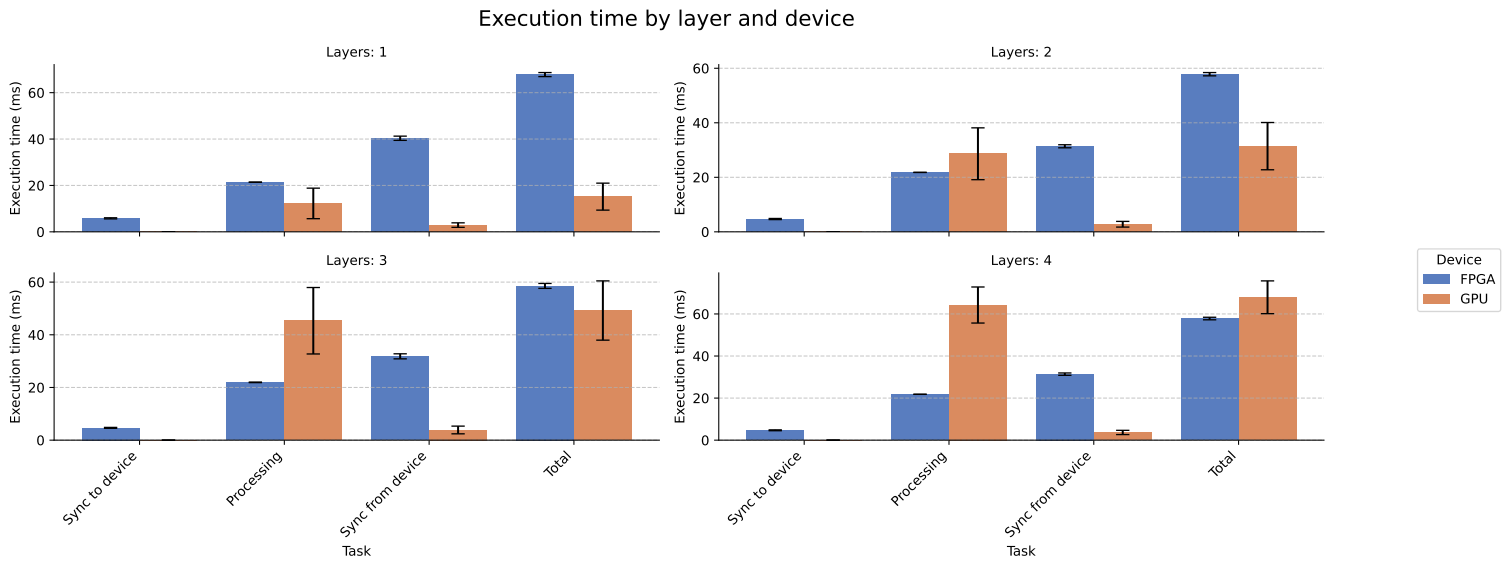
\includegraphics[width=0.9\textwidth]{fig/fpga_vs_jetson.png}
  \caption{\Gls{fpga} \Gls{snn} izpildes laiks salīdzinājumā ar ekvivalentu modeli GPU.}
  \label{fig:fpga_vs_jetson}
% \par\smallskip
% {\footnotesize \textit{Execution time by layer and device} — izpildes laiks pēc slāņu skaita un ierīces; \textit{Layers} — slāņi; \textit{Execution time} — izpildes laiks; \textit{Device} — ierīce; \textit{Sync to device} — sinhronizācija uz ierīci; \textit{Processing} — apstrāde; \textit{Sync from device} — sinhronizācija no ierīces; \textit{Total} — kopā; \textit{Task} — uzdevums.\par}
\end{figure}

Sekliem tīkliem abu platformu veiktspēja ir salīdzināma. Tomēr, palielinoties tīkla dziļumam, \Gls{fpga} konveijers tiek pilnībā noslogots un pārspēj GPU realizāciju. Novērtētajam četrslāņu tīklam kopējais inferences latentums saglabājas zem \qty{60}{\milli\second}, atbilstot reāllaika apstrādes prasībām automobiļu uztveres sistēmās.

Abās skaitļošanas platformās jaudas patēriņš uzraudzīts nepārtrauktas inferences slodzes laikā. \Gls{fpga} realizācijai \textit{Alpha Data} ražotāja nodrošinātā utilīta \texttt{avr2util} uzrādīja aptuveni 15,8~W paātrinātāja kartes jaudas patēriņu. \textit{Jetson AGX Orin} gadījumā uzraudzības utilīta \texttt{jtop} inferences laikā uzrādīja aptuveni 19,8~W, darbojoties 40~W jaudas režīmā. Tādēļ novērotā \Gls{fpga} kartes jauda pārbaudītajos apstākļos bija aptuveni par 20~\% mazāka nekā norādītā \textit{Jetson} jauda. Novērotā jaudas atšķirība jāuzskata par orientējošu pilnas ierīces līmeņa salīdzinājumu, kas ietver resursdatora sistēmas un perifērijas jaudu, nevis par tieši izmērītu \Gls{snn} paātrināšanas energoefektivitātes priekšrocību.
